\begin{figure}[htbp]
	\centering

	\begin{subfigure}[c]{0.3\textwidth}

		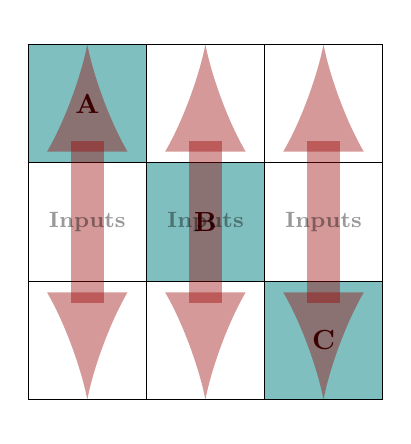
\begin{tikzpicture}

			\tikzstyle{interface}=[fill=white,draw=black,
				minimum width=1.5cm,minimum height=1.5cm,
				node distance=1.5cm]
			\tikzstyle{module}=[fill=teal!50,draw=black,
				minimum width=1.5cm,minimum height=1.5cm,
				node distance=1.5cm,
				align=center]

			\node[module]		(11)	{\bfseries A};
			\node[interface,right of=11]	(12)	{};
			\node[interface,right of=12]	(13)	{};
			\node[interface,below of=11]	(21)	{};
			\node[module,right of=21]		(22)	{\bfseries B};
			\node[interface,right of=22]	(23)	{};
			\node[interface,below of=21]	(31)	{};
			\node[interface,right of=31]	(32)	{};
			\node[module,right of=32]		(33)	{\bfseries C};

			\draw[red!60!black,line width=12pt,latex-latex,opacity=0.4]
				(11.north)  -- (31.south) 
				node[midway,text=black,font=\footnotesize\bfseries]{Inputs};
			\draw[red!60!black,line width=12pt,latex-latex,opacity=0.4]
				(12.north)  -- (32.south) 
				node[midway,text=black,font=\footnotesize\bfseries]{Inputs};
			\draw[red!60!black,line width=12pt,latex-latex,opacity=0.4]
				(13.north)  -- (33.south) 
				node[midway,text=black,font=\footnotesize\bfseries]{Inputs};
				
			\end{tikzpicture}

		\caption{N$^2$ inputs}
	\end{subfigure}
	\hfill
	\begin{subfigure}[c]{0.3\textwidth}

		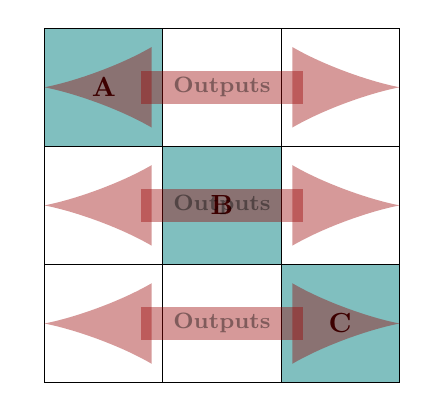
\begin{tikzpicture}
			
			\tikzstyle{interface}=[fill=white,draw=black,
				minimum width=1.5cm,minimum height=1.5cm,
				node distance=1.5cm]
			\tikzstyle{module}=[fill=teal!50,draw=black,
				minimum width=1.5cm,minimum height=1.5cm,
				node distance=1.5cm,
				align=center]

			\node[module]		(11)	{\bfseries A};
			\node[interface,right of=11]	(12)	{};
			\node[interface,right of=12]	(13)	{};
			\node[interface,below of=11]	(21)	{};
			\node[module,right of=21]		(22)	{\bfseries B};
			\node[interface,right of=22]	(23)	{};
			\node[interface,below of=21]	(31)	{};
			\node[interface,right of=31]	(32)	{};
			\node[module,right of=32]		(33)	{\bfseries C};

			\draw[red!60!black,line width=12pt,latex-latex,opacity=0.4]
				(11.west)  -- (13.east) 
				node[midway,text=black,font=\footnotesize\bfseries]{Outputs};
			\draw[red!60!black,line width=12pt,latex-latex,opacity=0.4]
				(21.west)  -- (23.east) 
				node[midway,text=black,font=\footnotesize\bfseries]{Outputs};
			\draw[red!60!black,line width=12pt,latex-latex,opacity=0.4]
				(31.west)  -- (33.east) 
				node[midway,text=black,font=\footnotesize\bfseries]{Outputs};

		\end{tikzpicture}

		\caption{N$^2$ outputs}
	\end{subfigure}
	\hfill
	\begin{subfigure}[c]{0.3\textwidth}

		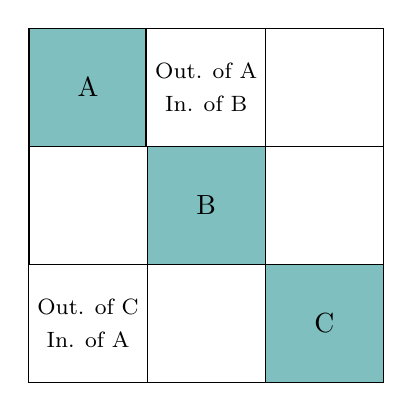
\begin{tikzpicture}
			
			\tikzstyle{interface}=[fill=white,draw=black,
				minimum width=1.5cm,minimum height=1.5cm,
				node distance=1.5cm,
				align=center]
			\tikzstyle{module}=[fill=teal!50,draw=black,
				minimum width=1.5cm,minimum height=1.5cm,
				node distance=1.5cm,
				align=center]

			\node[module]		(11)	{A};
			\node[interface,right of=11]	(12)	{\footnotesize Out. of A\\ \footnotesize In. of B};
			\node[interface,right of=12]	(13)	{};
			\node[interface,below of=11]	(21)	{};
			\node[module,right of=21]		(22)	{B};
			\node[interface,right of=22]	(23)	{};
			\node[interface,below of=21]	(31)	{\footnotesize Out. of C\\ \footnotesize In. of A};
			\node[interface,right of=31]	(32)	{};
			\node[module,right of=32]		(33)	{C};

		\end{tikzpicture}

		\caption{N$^2$ diagram}
	\end{subfigure}

	\caption{Example of a N$^2$ diagram}
	\label{fig:N2example}
\end{figure}

